\documentclass{beamer}

\title{some title}
\subtitle{subtitle}
\author{Troy Astorino, Neil Forrester}
\date{April 10, 2013}
\institute[6.834 -- MIT]{Cognitive Robotics \\ Massachusetts Institute of Technology}

\usepackage{graphicx}
\usepackage{amsmath}

\usetheme{CambridgeUS}
\usecolortheme{beaver}
\setbeamertemplate{section in toc}[square]
%\setbeamercolor{section number projected}[bg=black, fg=red]
\setbeamertemplate{navigation symbols}{} % remove navigation symbols

% \argmax operator
\DeclareMathOperator*{\argmax}{arg\,max}

% \norm{n}{stuff} is the L-n norm of stuff
\providecommand{\norm}[2]{\lVert#2\rVert_#1}

\newcommand{\overlay}[3]{\includegraphics<#3>[scale=#2]{img/#1.png}}
\newcommand{\overlayL}[2]{\overlay{#1}{0.5}{#2}}

% macros for including shape pictures at various scales (Large, Medium, Small)
\def \spL [#1]{\overlayL{#1}{1}}
\def \spM [#1]{\overlay{#1}{0.3}{1}}
\def \spS [#1]{\overlay{#1}{0.15}{1}}

\begin{document}

\begin{frame}
  \maketitle
\end{frame}

\begin{frame}
  \frametitle{Outline}
  \tableofcontents
\end{frame}

\section{section title}
\begin{frame}
  \frametitle{Why do we need manipulation-based search for occluded
    objects?}
  \begin{figure}
    \centering
    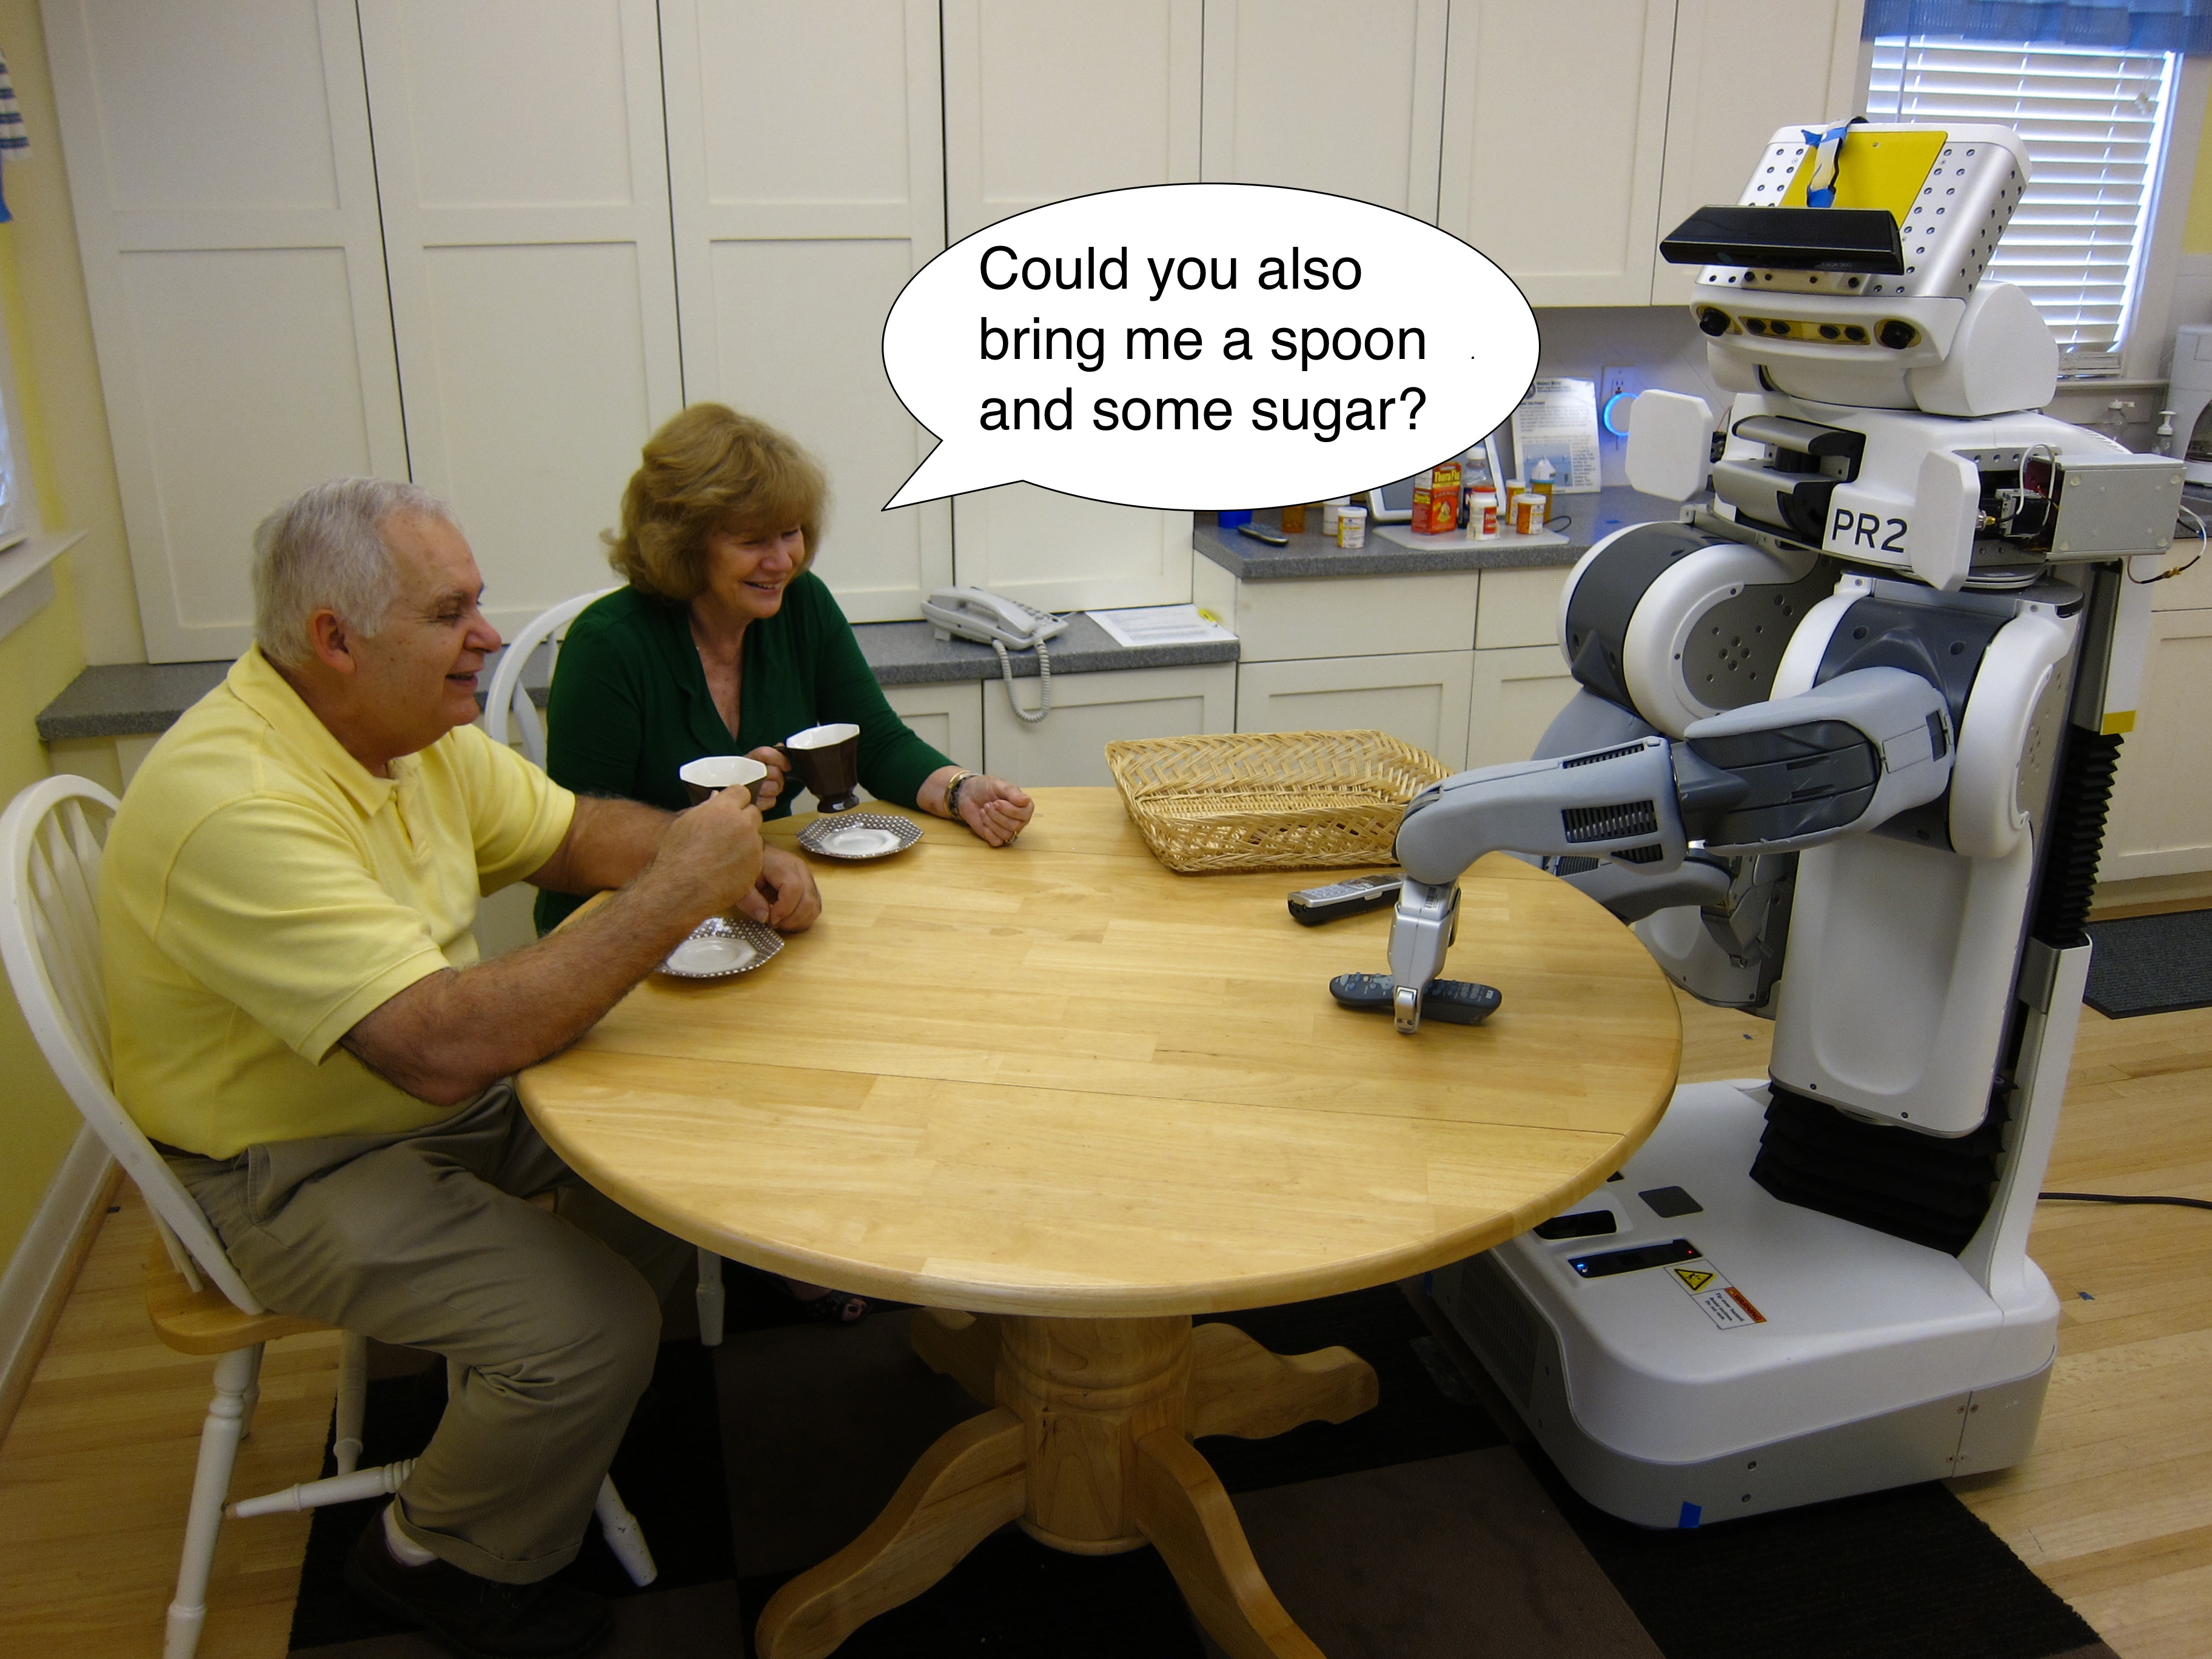
\includegraphics[width=3.2in]{img/robot_in_kitchen.jpg}

    \tiny{Original image courtesy of Wendy Rogers/Georgia Tech}
  \end{figure}
\end{frame}

\begin{frame}
  \frametitle{Assumptions for the following treatment}
  \begin{itemize}
  \item No errors in  visual identification and classification of objects
  \item Robot can successfully complete any movement and manipulation task, but
    these are temporally expensive
  \item Finite set of object types in the world
  \end{itemize}
\end{frame}

\begin{frame}
  \frametitle{Search planning}
  A robot searching for an object $q$ next removes an occluding object
  from the maximum likelihood container:

  \[\argmax_l{\mathbb{P}(q \in c_l|\{t_{o_j}\})}\]
  
  \begin{itemize}
  \item $c_l$ is the $l^{\text{th}}$ container
  \item $\{t_{o_j}\}$ is the set of observed objects
  \end{itemize}
\end{frame}

\section{Generative Model of Container Contents}
\begin{frame}
  \frametitle{The Problem}
  \begin{center}
    \vspace{-0.13in}
    Set of containers: $\{c_l\}$

    \spL[3-unknown-containers]

    Set of object types: $\{t_i\}$

    \spL[shape-universe-small]

    We want to find an object of type $q$ (the query type).

    \spL[blue-circle]

  \end{center}
\end{frame}

\begin{frame}
  \frametitle{Where is \spM[blue-circle]?}
  \begin{center}
    \spL[3-partially-observed-containers]

    \vspace{0.3in}

    Given that we have observed objects of types $\{t_{o_j}\}$ \\
    in container $c$, what is $\mathrm{P}(q \in c \, | \, \{t_{o_j}\})$ ?
  \end{center}
\end{frame}

\begin{frame}
  \frametitle{Composition of a container ($\theta$)}
  \begin{columns}
    \begin{column}{0.7\textwidth}
      \begin{center}
        \spM[shape-universe-small]\\
        \hspace{0.1in} 1 \hspace{0.2in} 2 \hspace{0.08in} 3 \hspace{0.08in} 4

        \begin{equation*}
          \theta' = (1, 2, 1, 3)
        \end{equation*}

        \begin{equation*}
          \theta = \frac{\theta'}{\norm{1}{\theta'}}
        \end{equation*}

        \begin{equation*}
          \theta = \Big ( \frac17, \frac27, \frac17, \frac37 \Big )
        \end{equation*}
      \end{center}
    \end{column}
    \begin{column}{0.3\textwidth}
      \spL[1-observed-container]
    \end{column}
  \end{columns}
\end{frame}



\begin{frame}
\frametitle{Packing a container}
\begin{center}
Want to calculate $\mathbb{P}(q \in c_l|\{t_{o_j}\})$ from samples of $\theta$

\[\theta\_samples = \left[ \left( 0.4, 0.2, 0.1, 0.3 \right),
                         \left( 0.2, 0.1, 0.3, 0.4 \right) \right]\]

\end{center}
\end{frame}

\begin{frame}
  \frametitle{Packing a container}
  \begin{columns}
    \begin{column}{0.7\textwidth}
      \begin{center}
        \vspace{-3em}

        \begin{align*}
          &\begin{aligned}
            \theta\_samples = [ & \left( 0.4, 0.2, 0.1, 0.3 \right), \\
            & \left( 0.2, 0.1, 0.3, 0.4 \right) ]
          \end{aligned} \\
          &\invisible<1,17>{i = \alt<1-8>{0}{\alert<9>1} \; \longrightarrow \; 
            \theta = \alt<1-8>{\left( 0.4, 0.2, 0.1, 0.3 \right)}
            {\alert<9>{\left( 0.2, 0.1, 0.3, 0.4 \right)}}}\\
          &count = \alt<1-7>{0}{\alert<8>{1}}, \; total = \temporal<8-16>{0}{\alert<8>1}{\alert<17>2}\\
        \end{align*}

      \item<2-6,10-15>{Shape sampled from $\theta$: \phantom{\hspace{5em}}}\\
      \overlayL{green-rectangle}{2}
      \overlayL{red-square}{3}
      \overlayL{blue-circle}{4}
      \overlayL{red-square}{5}
      \overlayL{green-rectangle}{6}
      \overlayL{red-square}{10}
      \overlayL{green-rectangle}{11}
      \overlayL{orange-triangle}{12}
      \overlayL{orange-triangle}{13}
      \overlayL{red-square}{14}
      \overlayL{orange-triangle}{15}

      \item<17>$\mathbb{P}(q \in c_l|\{t_{o_j}\}) = \frac12$

      \end{center}
    \end{column}
    \begin{column}{0.3\textwidth}
      \overlayL{container-packing-1-1}{1-2}
      \overlayL{container-packing-1-2}{3}
      \overlayL{container-packing-1-3}{4}
      \overlayL{container-packing-1-4}{5}
      \overlayL{container-packing-1-5}{6}
      \overlayL{container-packing-1-6}{7-8}
      \overlayL{container-packing-2-1}{9-10}
      \overlayL{container-packing-2-2}{11}
      \overlayL{container-packing-2-3}{12}
      \overlayL{container-packing-2-4}{13}
      \overlayL{container-packing-2-5}{14}
      \overlayL{container-packing-2-6}{15}
      \overlayL{container-packing-2-7}{16-17}
    \end{column}
  \end{columns}
\end{frame}

\end{document}
